\chapter{Předzpracování dat}


\section{Příprava mapových dat}
Nejprve jsou stažena aktuální data pro Českou republiku, která jsou k~dispozici
s~denními aktualizacemi.\footnote{\url{osm.kyblsoft.cz/archiv/}} Z~těchto dat je
na základě nastavení vyříznut obdélník, který pokrývá zpracovávanou oblast. Poté
začneme data zpracovávat.

Nejprve jsou klasifikovány jednotlivé objekty. Klasifikují se uzly, hrany a
multipolygony, jiné typy relací nejsou v~současné době používány. Každý objekt
je klasifikován nějakým typem podle toho, jaké má tagy. V~rámci konfigurace lze
přidělit nějakému tagu (buď samotnému klíči, nebo dvojici klíč-hodnota) určený
typ s~danou prioritou. Objekt bude mít typ daný pravidlem s~nejvyšší prioritou,
které jeho tagy splňují. Pokud objekt nesplňuje žádné pravidlo, získá speciální
typ označující neklasifikovaný objekt.V dalším zpracování se již nehledí na
původní tagy ale jen na typ, který daný objekt má.

Současně s~klasifikací typu objektu se stejným způsobem určují hrany, které se
nachází na mostech a uzly, které jsou v~podzemí. Klasifikovaná data nahrajeme do
databáze a další kroky provádíme jako databázové operace. 

\subsection{Dělení dlouhých linií}
Protože chceme hledat co nejblíže od výchozího zadaného bodu, v~případě dlouhých
rovných ulic, které jsou reprezentovány pomocí lomených linií s~dlouhými úseky
by se nám mohlo stát, že by nejbližší bod od hledaného místa neležel na ulici,
kde jsme, ale na nějaké sousední, od které nás dělí pás budov. Proto dlouhé
úseky cest rozdělíme na menší podúseky (viz obr. \ref{fig:deleni}), čímž tento problém eliminujeme.
Rozdělení se nám také bude hodit pro vytváření zkratek, o~kterých pojednáváme
níže.

\begin{figure}
  \centering
    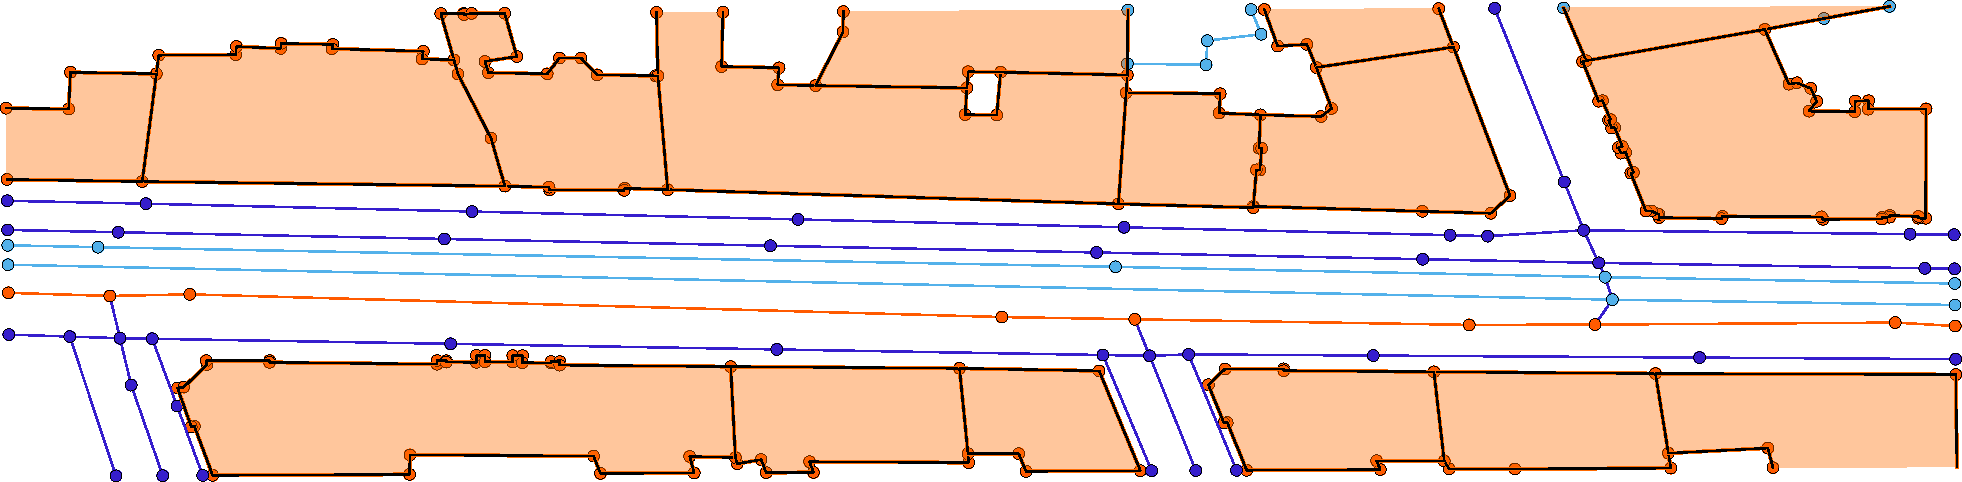
\includegraphics[width=0.75\textwidth]{../img/deleni.pdf}
  \caption{Rozdělení dlouhých linií (všimněte si, že jsou děleny jen pochozí
  linie)}
  \label{fig:deleni}
\end{figure}

\subsection{Překážky}
Pro další zpracování potřebujeme znát nejen cestní síť, ale i překážky, přes
které se nedá projít, jako jsou například domy, ploty a dálnice. V~tomto místě
se musíme vypořádat s~multipolygony. Protože multipolygony, které klasifikujeme
jako bariéry, jsou většinou budovy, které mají více částí nebo mají nádvoří,
nebo jiné překážky, uvnitř kterých neočekáváme velkou plochu, bereme
jako překážku jejich vnější obrys, případně obrysy. To nám sice způsobí, že
nebudeme moci vytvářet na vnitřních prostranstvích zkratky, ale to nám nevadí,
protože jednak mají vnitřní prostranství obvykle velmi malou plochu a nevede do
nich mnoho pěších cest, jednak vnitřní prostranství jsou buď zmapována
kompletně, nebo nedostatečně, tudíž by případné vytváření zkratek ve vnitřním
prostranství vedlo k~cestám, které by ve skutečnosti nebyly možné.

Výsledná množina překážek bude obsahovat vnější obrysy multipolygonů, další
polygonové objekty a liniové objekty.

\subsection{Body uvnitř objektů a body pod zemí}
Abychom mohli generovat zkratky, které budou průchozí i ve skutečnosti, je
potřeba určit, které body se nachází na volném prostranství na povrchu a které
se nacházejí pod zemí. Podzemní vrcholy jsme určili už v~rámci klasifikace.
Vrcholy uvnitř objektů jsme ztotožnili s~vrcholy, které se nachází uvnitř nějaké
překážky, protože překážky jsou pro nás takové objekty, přes které se nedá pěšky
projít napříč. Body, které se nacházejí na plášti překážky, jako vnitřní
neuvažujeme, protože se z~nich dá jít libovolným směrem, kde se nenachází
překážka.

\subsection{Zkratky}
Pro doplnění chybějících vazeb v~mapě používáme kromě cest v~mapových datech
již obsažených i automaticky generované zkratky. Zkratka spojuje dva pochozí
body na volném prostranství, které jsou nedaleko od sebe a úsečka mezi nimi,
reprezentující zkratku, neprotíná žádnou překážku. Dvojic bodů, které splňují
zadané podmínky, je ale velké množství a přidání všech zkratek by neúměrně
zvyšovalo velikost výsledných dat. Od určitého počtu zkratek z~daného vrcholu přidávání
dalších zkratek má jen malý vliv na délky hledaných cest, proto jsou ze všech
možných zkratek náhodně vybrány jen některé a to tak, aby z~každého vrcholu
vycházelo průměrně omezené množství zkratek. Takto zachováme pozitivní vliv
zkratek na hledané cesty, ale zbytečně nezvětšujeme vyhledávací graf.
\begin{figure}
  \centering
    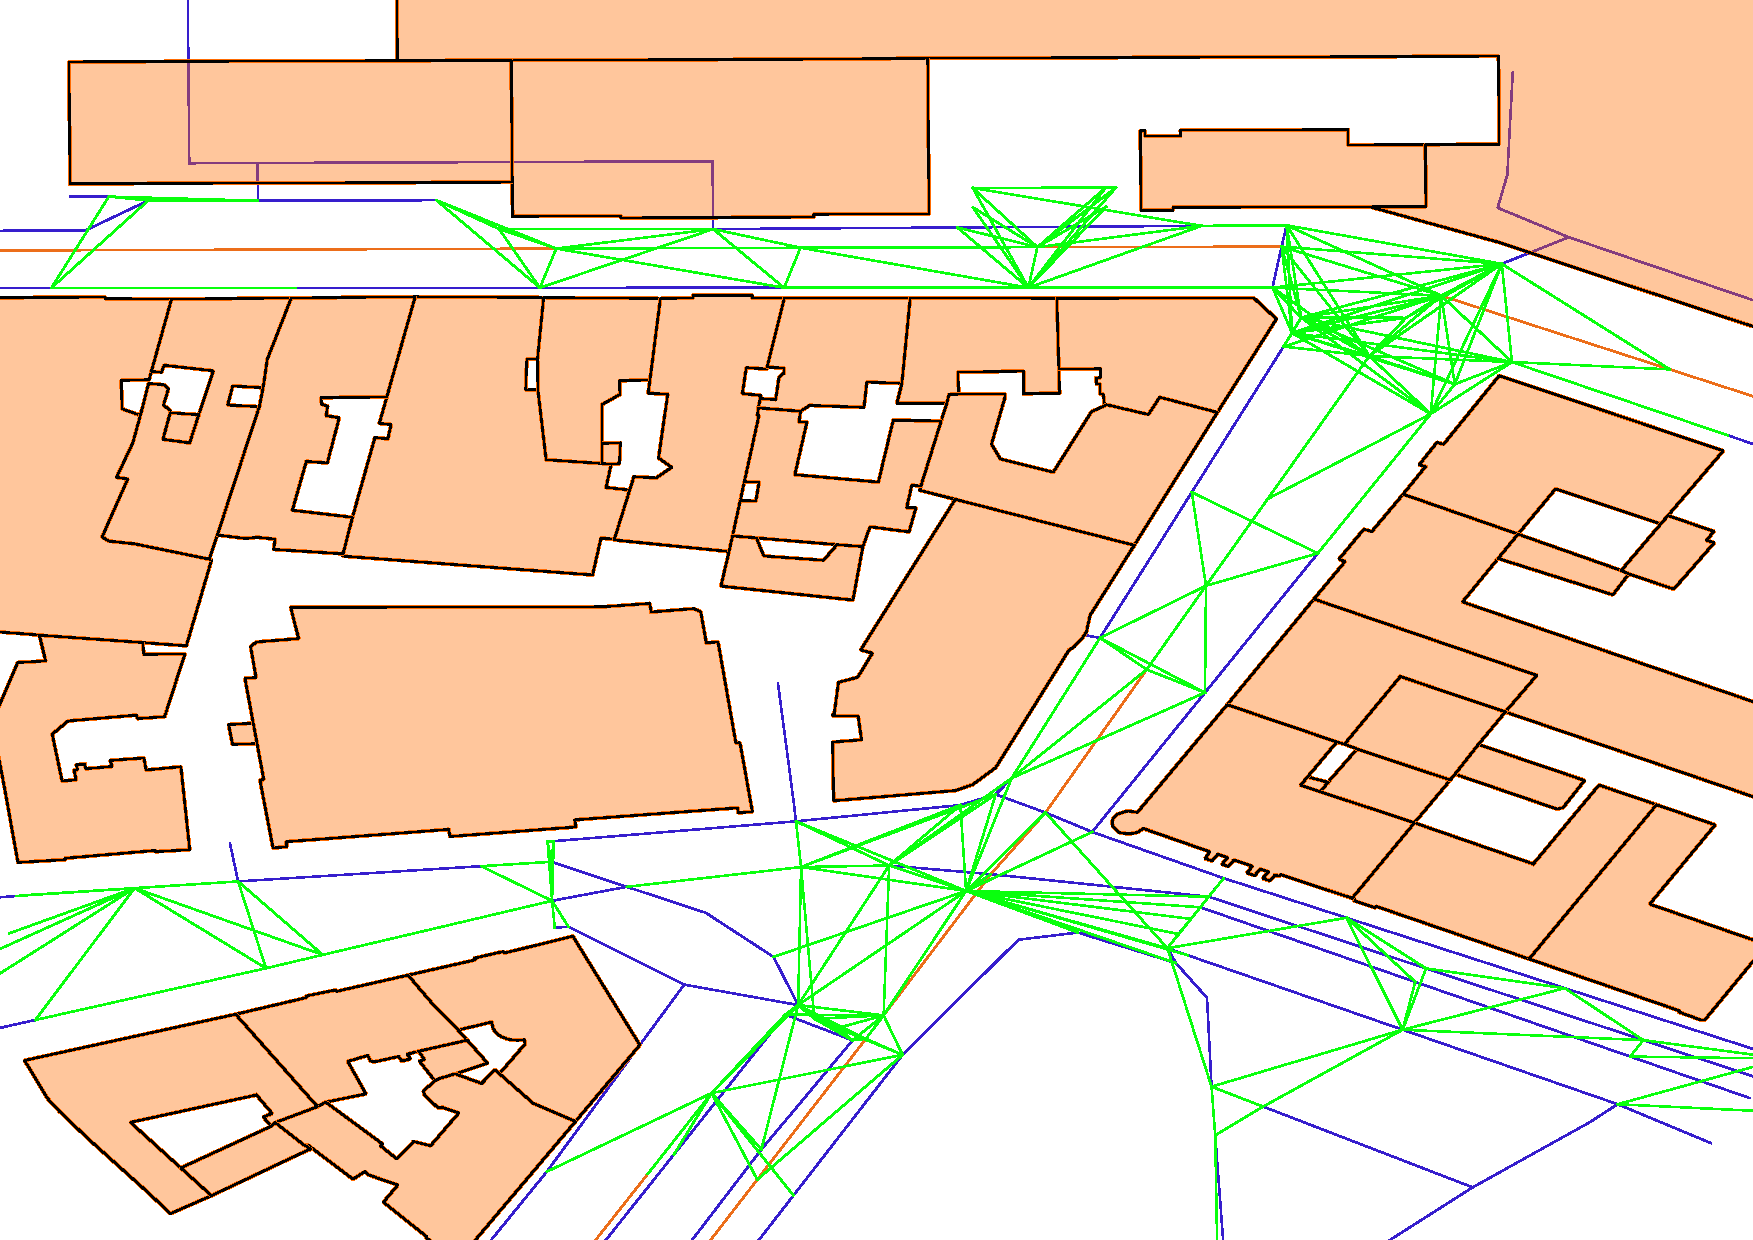
\includegraphics[width=0.5\textwidth]{../img/zkratky.pdf}
  \caption{Vygenerované zkratky mezi cestami (zeleně)}
  \label{fig:zkratky}
\end{figure}

\section{Příprava jízdních řádů}
Data z~jízdních řádů dostáváme ve formátu GTFS \cite{GTFS} a musíme je
upravit do formátu vhodného pro algoritmus RAPTOR \cite{RAPTOR}. V~rámci převodu
mezi formáty je potřeba respektovat specifické požadavky algoritmu RAPTOR a také
je potřeba připravit si informace potřebné pro propojení mezi zastávkami
v~jízdním řádu a zastávkami na mapě.

\subsection{Rozdělení linek}
Formát GTFS rozlišuje linky a spoje. Linka obsahuje všechny společné údaje a
jednotlivé spoje pak reprezentují jízdu vozidla dané linky mezi konkrétními
stanicemi, různé spoje jedné linky mohou projíždět různé posloupnosti stanic
(například spoje zatahující do vozovny, zkrácené vložené spoje, \dots).
Algoritmus RAPTOR ale vyžaduje, aby spoje konkrétní linky projížděly vždy
stejnou posloupnost zastávek. Abychom toho dosáhli, v~rámci předzpracování
najdeme všechny různé posloupnosti zastávek projížděné jednou linkou a vytvoříme
sublinky pro každou takovou posloupnost. Tyto sublinky zdědí společné údaje
z~původní linky a již splňují požadavky kladené algoritmem RAPTOR. 

\subsection{ID zastávek}
Zastávky mají dle specifikace GTFS jako ID použit obecný string. Data pro
pražskou MHD mají toto ID rozdělené na na část reprezentující zastávku a část
reprezentující konkrétní zastávkové stojany. Pro další zpracování je vhodné
zvolit číselný identifikátor, jednotlivé zastávky jsou očíslovány čísly od 0 do
počet zastávek $- 1$ a veškeré odkazy na konkrétní zastávky ve zpracovaných datech
používají právě tato čísla. Původní identifikátor je u~zastávky stále uložen
kvůli následnému párování (viz níže), ale již se pro vazbu mezi daty nepoužívá.

\subsection{Platnost jízdního řádu}
Ve formátu GTFS jsou linky, spoje a dny, ve kterých daný spoj jede, provázány
pomocí tabulky trips. V~předchozím odstavci jsme popsali rozdělení linek podle
toho, kudy spoje jedou, nyní využijeme, že každý spoj v~GTFS má právě jednu
množinu dní, kdy jede a tuto informaci si uložíme i u~jednotlivých spojů v~nově
vytvářeném formátu.

Místo dvojího způsobu záznamu, kdy daný spoj jede -- pomocí výčtu dnů v~týdnu a
seznamu výjimek -- si pro každou možnost, jak může nějaký spoj jet, uložíme
bitmapu platnosti a datum začátku a konce platnosti současného jízdního řádu. 
Bitmapa začíná první den platnosti a $i$-tý bit udává, zda i-tý den od začátku
platnosti daný spoj jede.  

\subsection{Podzemní stanice}
Při párování zastávek a pozic na mapě budeme potřebovat zvlášť ošetřovat
podzemní stanice, ze kterých se nelze vydat libovolným směrem, ale jen
eskalátorovým tunelem. V~rámci předzpracování označíme jako podzemní takové
zastávky, ve kterých jezdí metro. V~Praze takovýto předpoklad funguje správně,
protože všechny nadzemní stanice metra jsou zmapovány detailním způsobem, kdy
zpracování dat funguje korektně, pro jiná města s~jinou kvalitou zmapování by
bylo potřeba stanovit odlišná kritéria.


\section{Párování zdrojových dat}
Abychom moli plánovat spojení využívající jak pěší chůzi, tak jízdu MHD, je
potřeba data z~obou zdrojů vhodně provázat. Máme k~dispozici následující údaje:
\begin{enumerate}
\item OSM
\begin{itemize}
	\item jméno zastávky
	\item pozici zastávky
	\item ID zastávky (jen u~některých)
\end{itemize}
\item GTFS
\begin{itemize}
	\item jméno zastávky
	\item pozici zastávky
	\item ID zastávky
\end{itemize}
\end{enumerate} 
V~ideální případe by bylo možné spárovat zastávky jednoduše dle ID, bohužel
v~OSM má ID jen několik zastávek, většinu zastávek je tedy potřeba spárovat jinak.
Nabízelo by se párování podle pozic a jmen zastávek, ale bohužel zastávky v~GTFS
jsou výrazně posunuté oproti OSM i skutečnosti, navíc ne všechny zastávkové
stojany jsou v~OSM vyznačeny, zvláště tam, kde je několik zastávkových stojanů
za sebou, například v~autobusových terminálech. Pokoušet se párovat zastávky
v~GTFS pouze na zastávky v~OSM by bylo velmi náročné s~nejistým výsledkem.
Využíváme proto toho, že v~OSM máme zmapované nejen zastávky, ale i cesty a
zastávkám v~GTFS vytváříme speciální vrcholy dle jejich zeměpisné pozice v~GTFS
a pomocí zkratek je spojujeme s~nejbližšími cestami (viz Obrázek
\ref{fig:zastavka}. Bod reprezentující zastávku pak v~mapových datech označíme
jako zastávku.

\begin{figure}
  \centering
    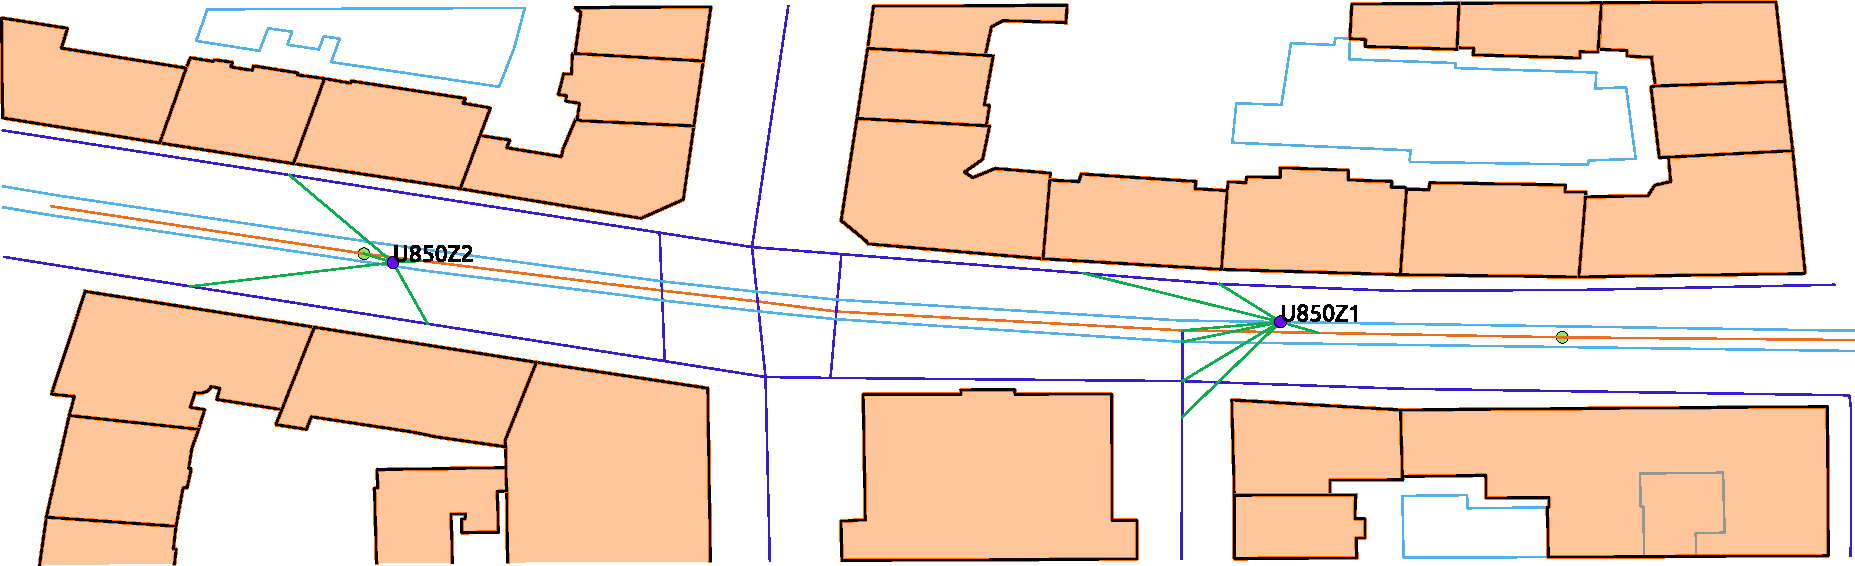
\includegraphics[width=\textwidth]{../img/tramvaj.pdf}
  \caption{Zkratky pro připojení tramvajové zastávky (zeleně)}
  \label{fig:zastavka}
\end{figure}

Pro zastávky z~GTFS, pro které máme v~OSM odpovídající ID, použijeme polohu
z~OSM a zkratky k~cestní síti hledáme z~této polohy. Zkratky jsou i zde potřeba,
protože dle pravidel OSM \cite{OSM} se zastávka umisťuje na místo, kde zastavuje
vozidlo, což například u~tramvají je bod na kolejích, které ale pro pěší
plánování nepoužíváme, tudíž je potřeba najít vhodný blízký bod v~cestní síti.

Zvláštní pozornost je potřeba věnovat u~párování zastávek metra. V~současné
chvíli je metro v~Praze zmapované dvěma způsoby. První způsob (viz obrázek 
\ref{fig:metro-detail}) je novější a
přesnější, jsou při něm zmapována nástupiště a eskalátorové tunely. Při tomto
podrobném mapování jsou také přidána ID stanic, tudíž je možné stanice jednoduše
spárovat a hledat cestu od hrany nástupiště. Častějším způsobem je ale starší
způsob (viz obrázek \ref{fig:metro-hrube}), kdy je stanice metra pouze bod, od
kterého vede eskalátorový tunel na
povrch. Tento eskalátorový tunel je pouze virtuální spojka, neodpovídá reálné
poloze podzemních tras. Takovéto stanice rovněž nemají přiřazená ID. U~těchto
stanic používáme polohu z~GTFS a zkratky spojující zastávku s~cestní sítí
hledáme do blízkých míst, která jsou v~podzemí, což vede k~poměrně dobré
aproximaci přístupu do metra. Jak bude postupovat mapování stanic metra, bude
tento typ stanic postupně eliminován a dojde ke zpřesnění navigace při
přestupech.

\begin{figure}
  \centering
    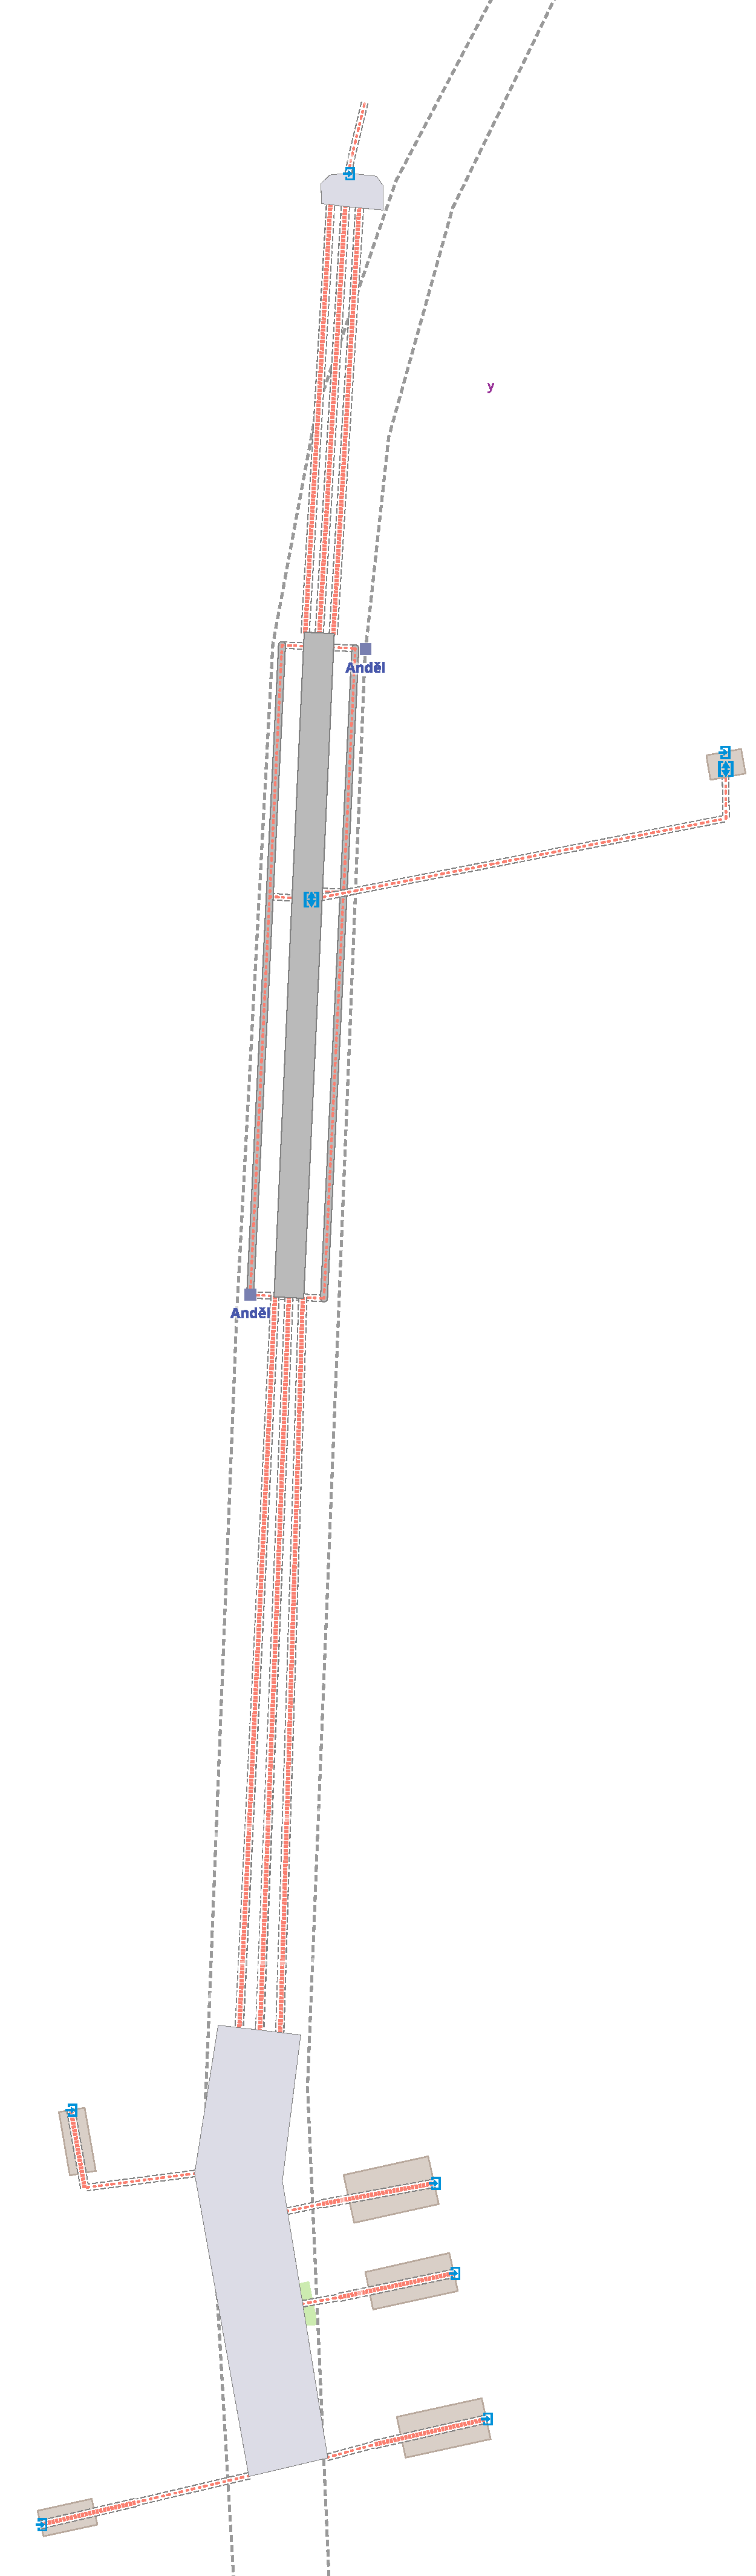
\includegraphics[height=0.98\textheight]{../img/andel.pdf}
  \caption{Detailně zmapovaná stanice metra Anděl}
  \label{fig:metro-detail}
\end{figure}

\begin{figure}
  \centering
    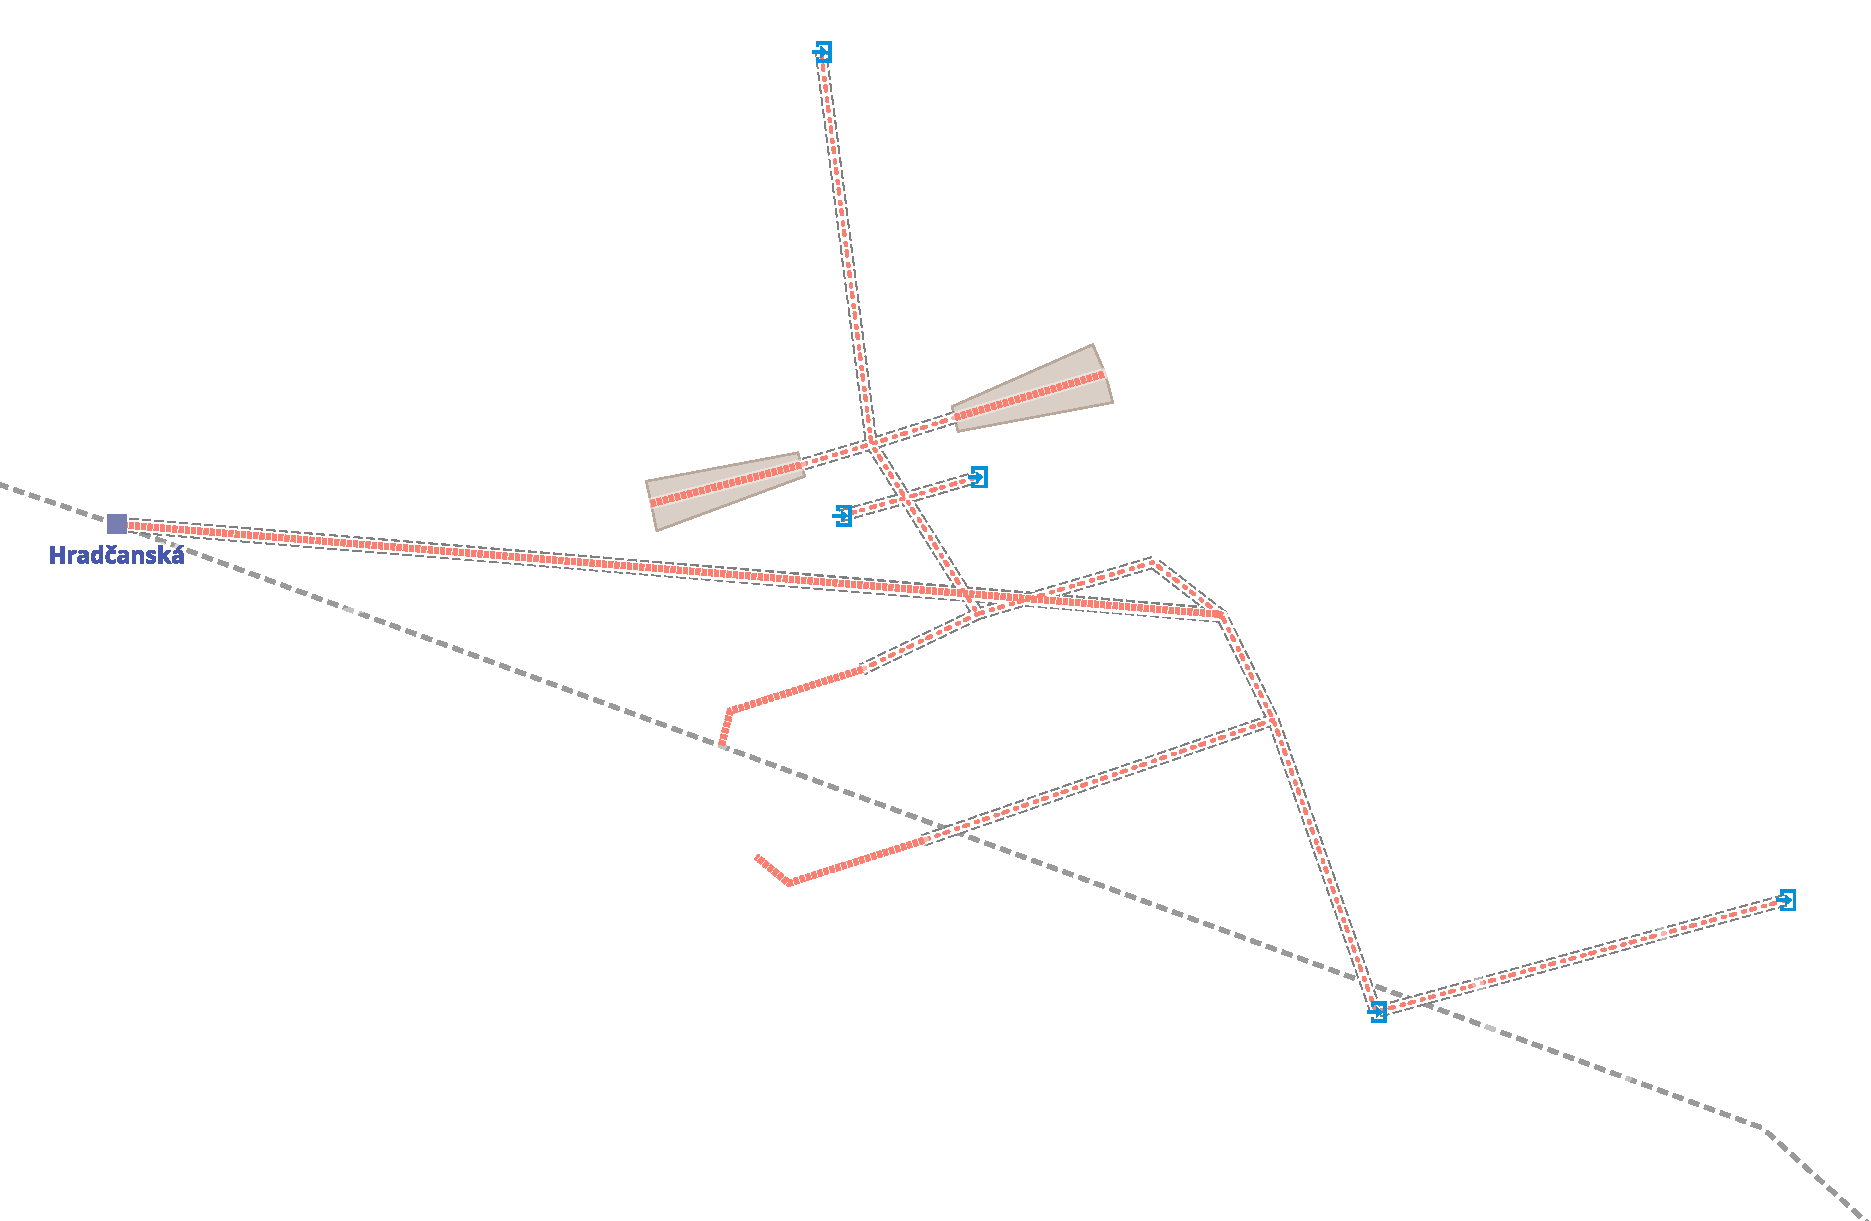
\includegraphics[width=\textwidth]{../img/hradcanska.pdf}
  \caption{Stanice metra Hradčanská zmapovaná starším způsobem}
  \label{fig:metro-hrube}
\end{figure}

Vždy jsou preferovány zastávky a stanice zmapované přesněji, které mají ID,
stačí tedy vylepšovat mapu a při dalším předzpracování dat se nově zmapované
zastávky dostanou i do vyhledávače.

